\documentclass[11pt]{article}

\usepackage[margin=1in]{geometry}
\usepackage[T1]{fontenc}
\usepackage[utf8]{inputenc}
\usepackage{lmodern}
\usepackage{graphicx}
\usepackage{booktabs,array}
\usepackage[nointegrals]{wasysym}
\usepackage[numbers,sort&compress]{natbib}

\usepackage{xcolor}

% Passages quoted verbatim in the response-to-reviewers letter are wrapped in
% \quoted{...} so they are easy to find when syncing the two documents.
% \showquotedtrue colours them; switch to \showquotedfalse for a clean
% submission PDF. Keep the colour in sync with response.tex's msquote.
\newif\ifshowquoted
% On by default. "make clean-pdf" builds unmarked PDFs by predefining
% \NOQUOTEDCOLOR on the pdflatex command line, so neither file has to be
% edited to produce a submission-ready copy.
\ifdefined\NOQUOTEDCOLOR\showquotedfalse\else\showquotedtrue\fi
\definecolor{quotedtext}{HTML}{7030A0}
\newcommand{\quoted}[1]{\ifshowquoted\textcolor{quotedtext}{#1}\else#1\fi}
\usepackage[hidelinks]{hyperref}
\usepackage[labelfont=bf,labelsep=period]{caption}
\newcommand{\botrule}{\bottomrule}

% Flat table of contents: every entry is one flush-left, dotted line.
\makeatletter
\renewcommand*{\l@subsection}{\@dottedtocline{1}{0pt}{0pt}}
\makeatother
\newcommand{\tocline}[1]{\addcontentsline{toc}{subsection}{#1}}
\providecommand{\bibcommenthead}{}

\renewcommand{\thefigure}{S\arabic{figure}}
\renewcommand{\thetable}{S\arabic{table}}
\renewcommand{\theHfigure}{S\arabic{figure}}
\renewcommand{\theHtable}{S\arabic{table}}
\setcounter{figure}{0}
\setcounter{table}{0}

\begin{document}

\title{\textbf{Supplemental Information for ``PoolParty: streamlined design of DNA sequence libraries in Python''}}

\author{%
Zhihan Liu$^{1}$, Aidan Cordero$^{1}$, Justin B. Kinney$^{1,*}$\\[0.75em]
{\small $^{1}$Simons Center for Quantitative Biology, Cold Spring Harbor Laboratory,}\\
{\small 1 Bungtown Rd., Cold Spring Harbor, New York 11724, United States}\\[0.5em]
{\small E-mail: \href{mailto:zhliu@cshl.edu}{zhliu@cshl.edu} (Z.L.),
\href{mailto:aicorder@cshl.edu}{aicorder@cshl.edu} (A.C.),
\href{mailto:jkinney@cshl.edu}{jkinney@cshl.edu} (J.B.K.)}\\[0.5em]
{\small $^{*}$Corresponding author}%
}

\maketitle

\renewcommand{\contentsname}{Contents}
\tableofcontents
\clearpage

\phantomsection
\tocline{\textbf{Supplemental Methods}}
\section*{Supplemental Methods}

\subsection*{Benchmarking analysis}
\quoted{Figure~\ref{fig:benchmark-scaling} and Table \ref{tab:benchmark-summary} present a benchmarking study of PoolParty using the three library designs featured in Figs.~2, 3, and 4 of the main text. Benchmarking experiments were run under Ubuntu 22.04.3 LTS in Windows Subsystem for Linux 2 on an Intel Core Ultra 9 185H workstation with 31~GB RAM allocated to WSL2, using CPython 3.12.2, PoolParty 0.1.0, and StateTracker 0.1.0. Timings are single-threaded wall-clock measurements of \texttt{generate\_library}, reported as mean $\pm$ SD over five replicate runs. Peak memory is the maximum resident set size reported by \texttt{getrusage}, with each data point measured in a fresh process.}

\subsection*{Tool comparisons}
\quoted{A literature search identified 13 tools with substantial functional overlap with PoolParty; these are listed in Table \ref{tab:tools}. Table \ref{tab:capabilities} compares the specific features and capabilities of the 7 tools most similar in purpose to PoolParty. Of these 7, we judged VaLiAnT \cite{Barbon2022th}, MPRAnator \cite{GeorgakopoulosSoares2017gb}, and tangermeme \cite{Schreiber2025nd} to be the closest competitors. MPRAnator is a web application that, as of this writing, is no longer accessible. Figs.~\ref{fig:valiant-comparison} and \ref{fig:tangermeme-comparison} provide explicit comparisons of the code/inputs required to construct identical libraries using PoolParty versus VaLiAnT (Fig.~\ref{fig:valiant-comparison}) or PoolParty versus tangermeme (Fig.~\ref{fig:tangermeme-comparison}). We note that neither VaLiAnT nor tangermeme is capable of generating all three libraries used in the benchmarking study of PoolParty.}

\clearpage

\begin{figure}[p]
\centering
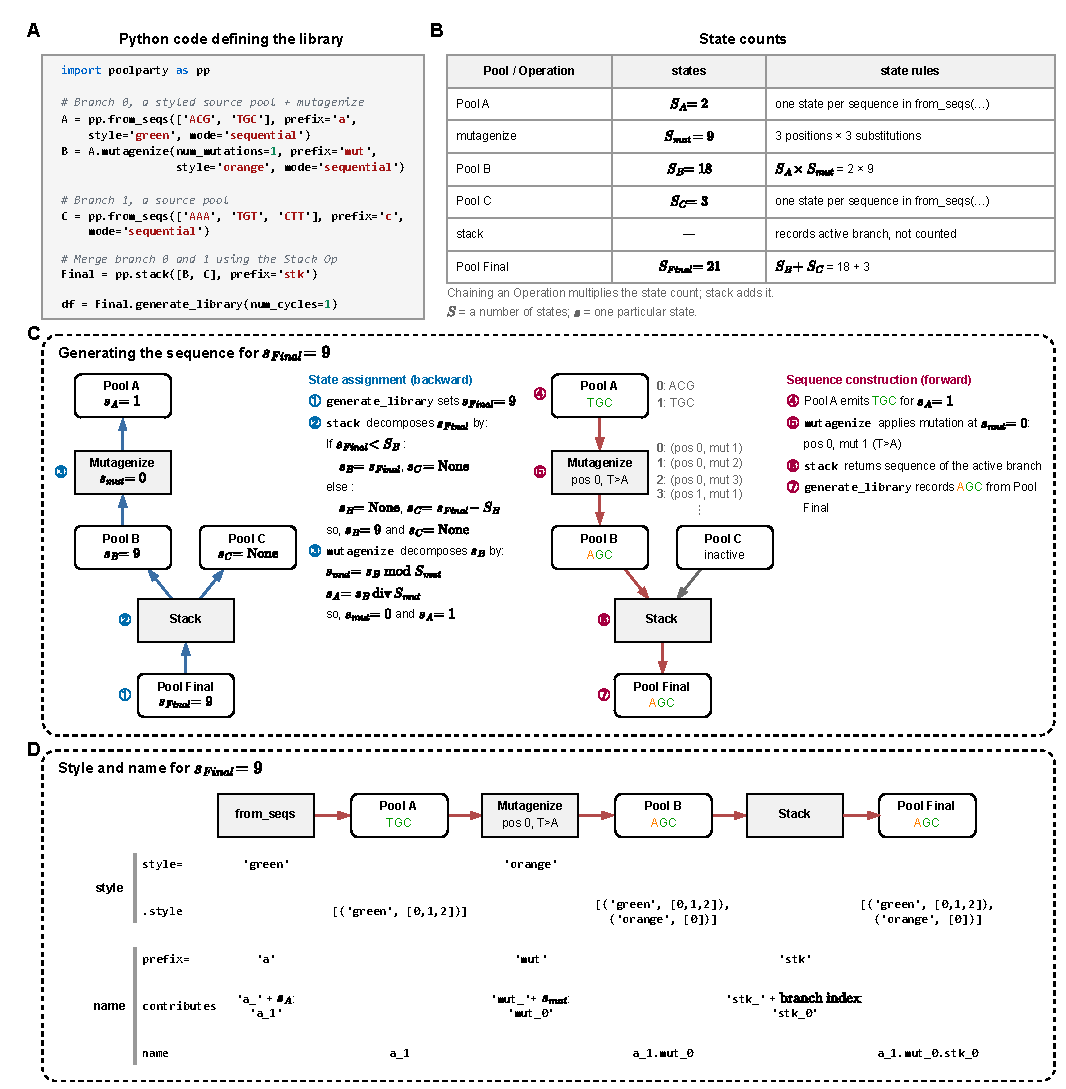
\includegraphics[width=\textwidth]{assets/figure_s1_sequence_generation}
\caption{\textbf{A worked example of sequence generation.} \textbf{(A)} Python code defining the DAG in Fig.~1B of the main text. \textbf{(B)} Number of states of each Pool and Operation. \textbf{(C)} Generating the sequence for $s_{Final} = 9$. Left: state assignment (blue). Right: sequence construction (magenta). Lists beside Pool A and \texttt{mutagenize} show which sequence or mutation each state selects. Inactive branches are shown in grey. \textbf{(D)} Style and name for the same sequence. Sequences are carried through the DAG as \texttt{Seq} objects, which hold the sequence string together with its \texttt{.style}. The \texttt{style} and \texttt{prefix} arguments are supplied to Operations; the resulting \texttt{.style} and name are held by Pools. Sequence characters are colored by their \texttt{.style} entries; where entries overlap, the last one applies. The styling shown in Panel D was generated by setting \texttt{\_include\_inline\_styles=True} in \texttt{Final.generate\_library()}; this is omitted from the code snippet in panel A.}
\label{fig:sequence-generation}
\tocline{\textbf{Figure S1.} A worked example of sequence generation}
\end{figure}

\clearpage

\begin{figure}[p]
\centering

\includegraphics[width=\textwidth]{assets/figure_s2_benchmark_scaling}
\caption{\textbf{Library generation scales linearly in time and memory.} \textbf{(A)} Wall-clock generation time, \textbf{(B)} throughput, and \textbf{(C)} peak resident memory against the number of sequences generated, for the three worked examples. Points are means of 5 replicate runs; error bars show $\pm$1~SD and are smaller than the plotting symbols at most points. Below $\sim$10$^3$ sequences a fixed setup cost dominates, giving the plateau in \textbf{(A)} and the rise in \textbf{(B)}; above 10$^4$ sequences throughput is constant, so generation time is linear in library size. Peak memory increases linearly, by 0.52--0.66~kB per sequence above a $\sim$106~MB baseline for the MPRA and SpliceAI libraries; similar behavior is observed for the GB1 library, but with a higher memory baseline.}
\label{fig:benchmark-scaling}
\tocline{\textbf{Figure S2.} Library generation scales linearly in time and memory}
\end{figure}

\clearpage

\begin{figure}[p]
\centering
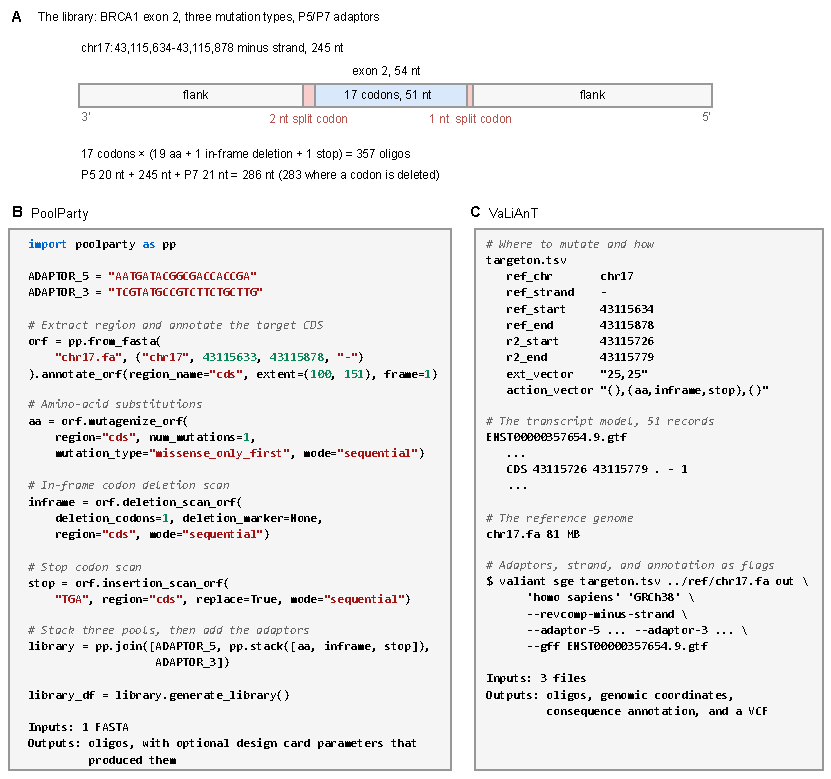
\includegraphics[width=\textwidth]{assets/figure_s3_valiant_comparison}
\caption{\textbf{The same BRCA1 exon 2 variant library in PoolParty and VaLiAnT.} \textbf{(A)} For each of the 17 complete codons in BRCA1 exon 2, the library contains substitutions to the other 19 amino acids, one stop-codon substitution, and one in-frame codon deletion. This gives 357 oligos. The split codons at the exon boundaries are left unchanged, and P5 and P7 adaptors are added to each sequence. \textbf{(B)} PoolParty implementation. The reference sequence is loaded from a FASTA file, and the user supplies the extent and reading frame of the 17 complete codons. Three ORF-aware Operations generate the amino-acid, stop-codon, and deletion scans. \textbf{(C)} VaLiAnT 4.0.0 implementation. VaLiAnT takes a coordinate and action table, a GTF annotation, and the reference chromosome as input. VaLiAnT gets the CDS phase from the GTF; in PoolParty, the user supplies the ORF extent and frame. The PoolParty code additionally calls \texttt{pp.set\_genetic\_code(valiant\_codon\_preference())} to match VaLiAnT's arginine codon choice; this setup line is omitted from panel B. When configured to use the same codon usage table, PoolParty and VaLiAnT gave exactly the same set of 357 sequences.}
\label{fig:valiant-comparison}
\tocline{\textbf{Figure S3.} The same BRCA1 exon 2 variant library in PoolParty and VaLiAnT}
\end{figure}

\clearpage

\begin{figure}[p]
\centering
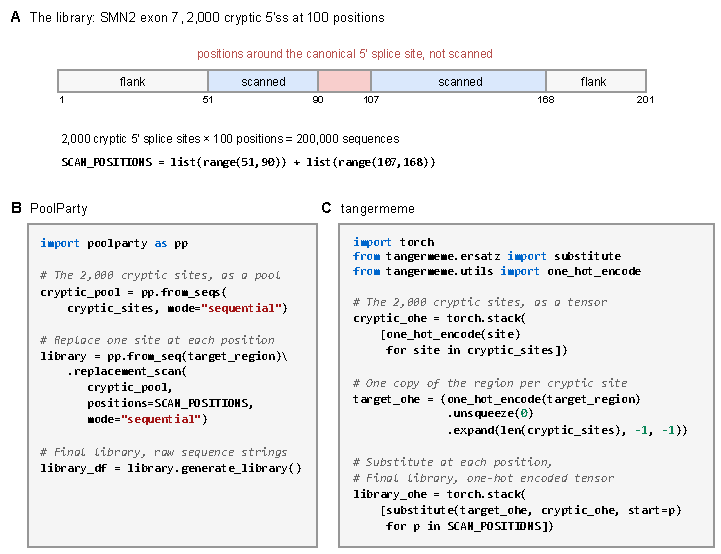
\includegraphics[width=\textwidth]{assets/figure_s4_tangermeme_comparison}
\caption{\textbf{The same cryptic splice-site perturbation library in PoolParty and tangermeme.} \textbf{(A)} The library contains 2,000 cryptic 5$'$ss 9-mers, each substituted at 100 positions across a 201-bp region containing the canonical 5$'$ss of SMN2 exon 7, giving 200,000 sequences. Positions immediately around the canonical site are excluded. This is the GT arm of the library in main-text Fig.~4; the matched control arm is built the same way. \textbf{(B)} PoolParty implementation. The 2,000 sites form a Pool, and \texttt{replacement\_scan} substitutes them at the 100 positions. The generated sequences are returned as strings in a table. \textbf{(C)} tangermeme 1.4.1 implementation. The target region and cryptic sites are one-hot encoded, substitutions are applied in one batch per position, and the final output is a tensor. After decoding this tensor, the two implementations gave the same set of 200,000 sequences.}
\label{fig:tangermeme-comparison}
\tocline{\textbf{Figure S4.} The same cryptic splice-site perturbation library in PoolParty and tangermeme}
\end{figure}

\clearpage

\begin{table}[p]
\centering
\footnotesize
\caption{\textbf{Runtime and memory for the three worked examples.} Each example was generated at the size shown using a single core. Generation times are means $\pm$ SD over five replicate runs. Peak memory is maximum resident set size and includes the fixed memory used by Python and the example DAG. DAG construction does not depend on library size and is reported separately. The SpliceAI library comprises two matched 200,000-sequence pools (cryptic GT and disrupted GA) generated separately; values are for one pool, and the full library takes twice as long.}
\label{tab:benchmark-summary}
\tocline{\textbf{Table S1.} Runtime and memory for the three worked examples}
\begin{tabular}{@{}lrrrrr@{}}
\toprule
Example & Library size & Time (s) & Sequence/s & Memory (MB) & DAG (s)\\
\midrule
GB1 deep mutational scan & 547,230 & $132.24 \pm 5.76$ & 4,138 & 487 & 0.22\\
MPRA regulatory grammar & 24,000 & $9.22 \pm 0.22$ & 2,602 & 127 & 0.06\\
SpliceAI surrogate & 200,000 & $11.93 \pm 0.27$ & 16,758 & 208 & 0.05\\
\botrule
\end{tabular}
\end{table}

\clearpage

% Supplementary tool overview. This file is the rendered deliverable;
% design decisions are recorded in table1.md.
% Requires: booktabs, array
% Individually listed tools are alphabetical; two grouped rows follow.
% PoolParty is bold, not first.
\begin{table}[tbp]
\centering
\scriptsize
% (setspace override omitted: measured to have no effect inside this float)
\setlength{\tabcolsep}{3pt}
\renewcommand{\arraystretch}{0.9}
\caption{\textbf{Tools for designing DNA sequence libraries and for related sequence-design problems.} The final two rows group related tools; their members are named and cited individually.}
\label{tab:tools}
\tocline{\textbf{Table S2.} Tools for designing DNA sequence libraries and related problems}
\begin{tabular}{@{}>{\raggedright\arraybackslash}p{2.0cm}>{\raggedright\arraybackslash}p{3.4cm}>{\raggedright\arraybackslash}p{4.3cm}>{\raggedright\arraybackslash}p{2.15cm}@{}}
\toprule
\textbf{Tool} & \textbf{Purpose / availability} & \textbf{Key features} &
\textbf{Output}\\
\midrule

MPRA Design Tools \citep{Ghazi2018aa} &
Design MPRA libraries and estimate statistical power. R package (GitHub). &
Barcode assignment with error-correcting sets; power analysis over effect size and sequencing depth &
Barcoded constructs and statistical power estimates\\
\addlinespace

MPRAnator \citep{GeorgakopoulosSoares2017gb} &
Design MPRA libraries of motif arrangements and sequence variants. Web service. &
Combinatorial placement of motifs; randomly sampled and combinatorial substitution sets; scrambled and reverse-complement controls &
Barcoded library of sequences (FASTA)\\
\addlinespace

Mutation Maker \citep{Hiraga2021yg} &
Design mutagenic oligos for building variant libraries in the laboratory. Web application (Docker); REST API. &
Degenerate codons at user-listed sites; several substitutions combined in one reaction; de novo gene assembly with per-site variant frequencies &
Primers, or gene fragments with the proportion of each variant to pool\\
\addlinespace

Oligopool Calculator \citep{Hossain2024oc} &
Add barcodes, primers, and spacers to a supplied variant set, and analyze the sequencing readout. Python package (PyPI); command line. &
Constraint-aware barcodes, primers, and spacers; degenerate compression of a supplied variant set; off-target screening against a host genome &
Synthesis-ready constructs; variant counts from sequencing reads\\
\addlinespace

\textbf{PoolParty} &
Design libraries that combine multiple variant types for laboratory assays or for probing genomic AI models. Python package (PyPI). &
Libraries specified as a directed acyclic graph of Operations and Pools, allowing different mutagenesis schemes to be combined; sequences generated only on request &
Library of sequences, each paired with a record of how it was constructed\\
\addlinespace

tangermeme \citep{Schreiber2025nd} &
Generate perturbed sequence sets to probe cis-regulatory logic in deep learning models. Python package (PyPI). &
Saturation mutagenesis of input sequences; insertion and removal of motifs across sets of sequences &
Perturbed sequences, model predictions, or attribution scores\\
\addlinespace

VaLiAnT \citep{Barbon2022th} &
Design and annotate libraries for saturation genome editing and cDNA deep mutational scanning. Command-line tool (source, Docker). &
Saturation mutagenesis from genomic coordinates; several mutation types per target region; transcript-aware, including codons split across exons &
Per-region libraries with metadata tables and VCF carrying variant consequence annotation\\
\midrule

General-purpose toolkits\newline\textit{(Biopython, pydna, SeqPro)} \citep{Cock2009df,Pereira2015wj,Klie2023kg} &
Manipulate sequences, simulate cloning, prepare arrays for modeling. Python packages (PyPI). &
Parsing, transformation, and file-format support &
Transformed sequences\\
\addlinespace

Sequence optimization tools\newline\textit{(CodonGenie, DNA Chisel, ledidi)} \citep{Swainston2017rb,Zulkower2020jk,Schreiber2025ledidi} &
Optimize individual sequences for codon usage, synthesis constraints, or a model's objective. Python packages (PyPI); web services. &
Degenerate codons covering a target residue set; hard constraints and scored objectives combined in one problem; gradient-based editing guided by a predictive model &
An optimized or edited sequence, or a degenerate codon\\
\botrule
\end{tabular}
\end{table}


\clearpage

% Table 2 - capability matrix. GENERATED from MATRIX.md - do not hand-edit.
% Column headers: 45deg. origin=lB anchors each label at its own baseline-left,
% so all labels share one baseline; \makebox[0pt][l] gives them zero width so
% they add nothing to the table and cannot overflow the line. Each label then
% starts at its column center and runs up-right. tabcolsep is 10pt so adjacent
% diagonals clear each other (~19pt perpendicular separation).
% A 3pt left nudge (about half a symbol width) sets each diagonal over the
% middle of its column of symbols rather than flush with the left edge.
% Measured: 0.00pt baseline stagger, uniform -3.5pt offset, no overfull.
% Requires: booktabs, graphicx, wasysym (\usepackage[nointegrals]{wasysym})
\newcommand{\hbfull}{\CIRCLE}
\newcommand{\hbhalf}{\LEFTcircle}
\newcommand{\hbnone}{\Circle}
\begin{table}[tbp]
\centering
\footnotesize
% (setspace override omitted: no effect inside this float)
\setlength{\tabcolsep}{10pt}
\caption{\textbf{Capabilities of tools for designing DNA sequence libraries and for related sequence-design problems.} \hbfull\ denotes a capability the tool provides; \hbhalf\ one provided with restrictions; \hbnone\ one the tool does not provide. Capabilities are counted only where the tool provides a dedicated operation, parameter, or mode.}
\label{tab:capabilities}
\tocline{\textbf{Table S3.} Capabilities of tools for designing DNA sequence libraries and related problems}
\begin{tabular}{@{}lcccccccc@{}}
\toprule
& \makebox[0pt][l]{\hspace*{-3pt}\rotatebox[origin=lB]{45}{DNA Chisel}} & \makebox[0pt][l]{\hspace*{-3pt}\rotatebox[origin=lB]{45}{MPRA Design Tools}} & \makebox[0pt][l]{\hspace*{-3pt}\rotatebox[origin=lB]{45}{MPRAnator}} & \makebox[0pt][l]{\hspace*{-3pt}\rotatebox[origin=lB]{45}{Mutation Maker}} & \makebox[0pt][l]{\hspace*{-3pt}\rotatebox[origin=lB]{45}{Oligopool Calculator}} & \makebox[0pt][l]{\hspace*{-3pt}\rotatebox[origin=lB]{45}{\textbf{PoolParty}}} & \makebox[0pt][l]{\hspace*{-3pt}\rotatebox[origin=lB]{45}{tangermeme}} & \makebox[0pt][l]{\hspace*{-3pt}\rotatebox[origin=lB]{45}{VaLiAnT}}\\
\midrule
\multicolumn{9}{@{}l}{\textit{Library Specification}}\\
\quad Library object & \hbnone & \hbhalf & \hbnone & \hbhalf & \hbhalf & \hbfull & \hbhalf & \hbnone\\
\quad Composable operations & \hbhalf & \hbnone & \hbhalf & \hbnone & \hbfull & \hbfull & \hbhalf & \hbnone\\
\quad Mixed variant types in one library & \hbnone & \hbfull & \hbfull & \hbhalf & \hbnone & \hbfull & \hbnone & \hbfull\\
\addlinespace
\multicolumn{9}{@{}l}{\textit{Variant Generation}}\\
\quad Saturation mutagenesis & \hbnone & \hbnone & \hbnone & \hbnone & \hbhalf & \hbfull & \hbfull & \hbfull\\
\quad Randomly sampled variants & \hbfull & \hbhalf & \hbfull & \hbnone & \hbnone & \hbfull & \hbnone & \hbnone\\
\quad Pairwise and higher-order variants & \hbfull & \hbnone & \hbfull & \hbfull & \hbhalf & \hbfull & \hbhalf & \hbnone\\
\quad Model-guided variants & \hbfull & \hbnone & \hbnone & \hbnone & \hbnone & \hbhalf & \hbfull & \hbnone\\
\addlinespace
\multicolumn{9}{@{}l}{\textit{Variant Types}}\\
\quad Codon / amino-acid substitutions & \hbfull & \hbnone & \hbnone & \hbhalf & \hbnone & \hbfull & \hbnone & \hbfull\\
\quad Insertions and deletions & \hbnone & \hbfull & \hbhalf & \hbnone & \hbnone & \hbfull & \hbfull & \hbfull\\
\quad Combinatorial multi-motif placement & \hbnone & \hbnone & \hbfull & \hbnone & \hbnone & \hbfull & \hbfull & \hbnone\\
\quad Recombination & \hbnone & \hbnone & \hbnone & \hbnone & \hbnone & \hbfull & \hbnone & \hbnone\\
\quad Shuffling & \hbnone & \hbnone & \hbhalf & \hbnone & \hbnone & \hbfull & \hbfull & \hbnone\\
\addlinespace
\multicolumn{9}{@{}l}{\textit{Physical Construction}}\\
\quad Synthesis-constraint checking & \hbfull & \hbhalf & \hbhalf & \hbnone & \hbfull & \hbhalf & \hbnone & \hbhalf\\
\quad Constraint-based optimization & \hbfull & \hbhalf & \hbhalf & \hbfull & \hbfull & \hbnone & \hbnone & \hbnone\\
\quad Primer design & \hbhalf & \hbnone & \hbnone & \hbfull & \hbfull & \hbnone & \hbnone & \hbnone\\
\addlinespace
\multicolumn{9}{@{}l}{\textit{Metadata and Inspection}}\\
\quad Per-sequence construction records & \hbfull & \hbfull & \hbhalf & \hbfull & \hbfull & \hbfull & \hbnone & \hbfull\\
\quad Automatic naming & \hbnone & \hbhalf & \hbfull & \hbfull & \hbhalf & \hbfull & \hbhalf & \hbfull\\
\quad Sequence styling & \hbnone & \hbnone & \hbhalf & \hbnone & \hbnone & \hbfull & \hbnone & \hbnone\\
\addlinespace
\multicolumn{9}{@{}l}{\textit{Genomic Integration}}\\
\quad Genome coordinates & \hbnone & \hbhalf & \hbfull & \hbnone & \hbnone & \hbhalf & \hbhalf & \hbfull\\
\quad Transcript / annotation aware & \hbnone & \hbnone & \hbnone & \hbnone & \hbnone & \hbnone & \hbnone & \hbfull\\
\botrule
\end{tabular}
\end{table}

\clearpage

\phantomsection
\tocline{\textbf{References}}
\bibliographystyle{sn-vancouver-num}
\bibliography{references}

\end{document}
